% !TEX root = ../main.tex

\chapter{Blockchain Audits: from Existence to Internal Controls} \label{sec:auditing} 

% \chapter{Blockchain Audits: from Smart Contracts to Cryptoassets} \label{sec:auditing} %TODO: or should we change all to Crypto Assets, with the space

% \chapter{Blockchain Audits: from Financial Statements to Smart Contracts} \label{sec:auditing}


% Older Drafts:
% - https://docs.google.com/document/d/1kay4MN97oEe8Hq_ESLyeFEYQ1BFnt7CA4SO0i6TasAU/edit#heading=h.xcne92a7aokg
% - https://docs.google.com/document/d/1MMlfDHH6rOtvKPIYJ0UQzXW9Of-vWJTRC6O7tqOJy50/edit
% - https://docs.google.com/document/d/1vlz2QOKa_iDTLcCUUcuRHBAaGmDVmKpnP3C3E4Av5Y8/edit
% - How to audit ERC20: https://docs.google.com/document/d/1EnvfnycZTe8250hn_MXCHCHR5CX2aZ0N09VUGYEROH0/edit#heading=h.9rrk8q89waxs

% Newer draft bulletpoints: https://github.com/MadibaGroup/2023-DAudit



\begin{quote}
	\textit{This chapter is based on the paper ``Systemizing the Challenges of Auditing Blockchain-Based Assets''~\cite{pimentel2021systemizing} published in the American Accounting Association Journal of Information Systems (JIS 2021, Volume 35, Issue 2). This paper was co-authored with Erica Pimentel, and supervised by Jeremy Clark and Emilio Boulianne. This chapter is partially rewritten to emphasize my individual contributions to the subject.}
	% TODO: change this to reflect the contribution and modifications
\end{quote}



\section{Introduction} \label{sec:auditing:intro}

In the previous chapters, we looked at several subtle technical issues with how a blockchain works and its limitations. The main conclusion is that if mis-understood or not mitigated, such issues can result in unforeseen consequences. These consequences can bring harm to the company behind the technology, the open source community developing it, and the users. Protecting users is important to government regulators, and protecting businesses is important to both regulators and to investors with a financial stake in the business. 

One tool used by investors and regulators to protect businesses is to oblige or mandate it to undergo an audit of its financial position, as conducted by a highly regulated and arms-length audit firm. Another tool that is typically not legally mandated, but is often demanded by users and investors, is a technical audit of all protocols and software used in the solution. These two types of audits are not mutually exclusive. Financial auditors may take into consideration the results of technical audits when assessing the risks of a company holding blockchain-based assets or deriving profits from blockchain-based services. 

The purpose of this chapter is to showcase one way the (occasionally theoretical or hypothetical) examples given in the previous chapters actually matter in the real world. Throughout this chapter, we focus on the financial audit of the crypto-assets on a company's balance sheet, as opposed to the technical audit (\eg security code review) of the smart contracts servicing these assets. However, we will consider both and conclude that they overlap---the technical audit of the smart contracts can be used as a tool to assist the financial auditors in their process (\eg Section~\ref{sec:auditing:case-studies:ownership}).

Our research has uncovered that major accounting firms are hesitating to provide certification in the blockchain sector due to a perception of insurmountable business risk associated with these clients. Auditors believe that due to a complex and rapidly changing technological environment, they have yet to develop the in-depth knowledge of their clients' blockchain businesses in order to perform an audit. Due to the lack of guidance, standards and regulations in this space, auditors are reticent to take on new clients in a sector that has been subject to numerous frauds~\cite{abreu2018blockchain}. Accordingly, the inability to obtain audited financial statements presents a key barrier to investment and growth in the blockchain sector. 

Put plainly, should the subtle risks we repeatedly illustrate in Chapters 3--5 frighten an auditor, who generally will not have deep technical knowledge, and cause them to avoid any company with crypto-assets on their balance sheet? This chapter aims to bring forth issues associated with auditing blockchain-based assets by making parallels to traditional financial statement audits. We cannot answer this conclusively, however our research points to several paths forward, which we compare.


% ConsenSys diligence work —> borrow from auditing paper with Erica, illusion of chapter is paper reviewed but adding the framework of the existence, evaluation, ownership, internal control weave in stuff from code review and and CTO stuff. (no on the interviews)

% shine on what people do, for crypto auditing. <— (wait on Jeremy for a paper)
% —> what is manual audit, you still need it. framwork of the OEInternal controls, what could go wrong ! what about airdrops for the balance, get from the vasanth paper add stuff
% what can be done 
% borrow from the FC version auditing paper <— 


% Based on published work but my opinions?

% Financial audit <> code review audit


%++++++++++++++++++++++=======================================+++++++++++++++++++++

\section{Background and Motivation} \label{sec:auditing:background}

\subsection{Financial Audits}

In certain common circumstances, firms operating in the blockchain space will require their financial statements to be audited by an external firm. Annual audits are legally mandatory for publicly traded companies in most countries, and audits might also be required when a firm borrows from a bank or raises capital from investors. Auditing is performed by a third party, who is independent of the firm being audited. The auditor's role is to provide an opinion on the financial statements of the firm, and to provide reasonable assurance that the financial statements are free of material misstatements or undeclared risks. The auditor's opinion is based on the audit evidence obtained during the audit process.

The blockchain industry is composed of firms (raising more than \$15B in unregulated funding and \$2.5B in venture capital in 2018~\cite{coindesk2018}) that issue and manage cryptoassets (worth a combined \$1.64T at the time of writing~\cite{coinmarketcap}). While this market is experiencing rapid growth, it is dominated by startups that lack the financial sophistication and maturity of similarly valued traditional firms, and that rely on outside funding to develop and grow. These small firms will require audited financial statements to obtain traditional forms of credit such as bank loans or to gain access to public markets. For instance, SEC registrants must file audited financial statements that have an unqualified audit opinion (except under limited circumstances)~\cite{securities2009financial}. If registrants are unable to provide unqualified audited statements, they will be unable to raise capital on public markets. 

At the time of writing, auditing firms are hesitant to provide audit opinions to the blockchain sector. Furthermore, several crypto companies such as Impak Finance (who undertook the first legal ICO in Canada~\cite{AMFImpactFinance}), Hut 8 Mining Corp., Vogogo Inc. and DMG Blockchain Solutions Inc., were placed on cease trade for failure to produce timely financial statements when their auditors abruptly stepped down and the companies were unable to find replacement auditors~\cite{posadzki2019crypto}. Therefore, the inability to obtain audited financial statements is a pressing issue as both new and existing firms are having difficulty finding auditing firms who wish to provide opinions to crypto companies.

\subsection{Cryptoassets}

We use the term cryptoasset and cryptoliability to refer to listings on a firm's balance sheet that exist and are transacted using blockchain technology and have some tradable value. This includes cryptocurrencies (e.g., bitcoin and ether) as well as tokens (\eg ERC20) issued by smart contracts running on a blockchain. Among others, the main categories of tokens are: (1) \textit{Access tokens}: a service is developed that requires its own custom tokens for using the service; (2) \textit{Backed tokens}: a token issuer claims to be holding something valuable (material or digital) in reserve, and the token represents a claim on these reserves; (3) \textit{Equity tokens}: a firm issues tokens to represent ownership shares of the company; and (4) \textit{Collectable tokens}: the token itself is offered as a contemporary collector's item. 

\subsection{Ethereum Address Types}

In Ethereum, there are two types of addresses: externally owned accounts (EOA) and smart contracts. An EOA is the equivalent of an address in Bitcoin. The address value itself is based on a hash of the user's public key. The address can be used to send a transaction, which is signed by the EOA's associated private key. 

Recall that Ethereum allows the creation of smart contracts. A smart contract is generally created by an EAO, as a special kind of transaction different from sending ETH (contracts can also create other contracts, which we generally do not consider here). During contract creation time, Ethereum designates an address for the contract. This value is derived pseudorandomly from details about the contract itself and thus does not have a corresponding private signing key. Thus anything done with the contract's address (such as sending ETH, tokens, calling functions on other contracts, \etc) must be coded into the functionality of the contract itself. At contract creation time, Ethereum copies the code of the contract into storage. The code is either provided directly or indirectly (through instructions that Ethereum can execute for obtaining a copy of the code). The code is stored at the contract address and the code cannot be changed with only one exception: executing the \texttt{selfdestruct} opcode. 

ETH and other assets sent the address of a smart contract cannot be transferred out of the contract without support from the code of the contract. Contracts typically implement access control, the simplest being the designation of a single EOA that can perform sensitive tasks like transacting the assets belonging to the contract's address. 

\subsection{Multisig}

A more involved access control pattern is a multi-signature (multisig) where more than one EOA (or contract address) must support the operation. For example, a multisig might require support from 7 of 12 addresses. There are different possible implementations and configurations on how each multisig smart contract can be set up~\cite{ittay2021wallet}.  
 
 An alternative to multisig is a threshold signature, where a single EOA is specified in the contract but off-chain, the signature has been set up such that 12 key-shares exist and any 7 of them is required to form a signature value~\cite{gennaro2018fast,zhao2019secure}. Thus, seeing a contract with a single EOA suggests but does not conclusively demonstrate single party control. Threshold signatures have one logistical drawback: the algorithm for creating the key shares generates a random share (so that it has the correct mathematical structure). Say Alice is participating in two different access control groups, only with multisig can she use the same EOA in both groups. Next assume Alice is a smart contract address (for example, wallet software like Gnosis Safe). Since contracts are assigned address values by Ethereum and have no corresponding public key, they cannot be used with a threshold signature scheme. They also cannot be directly used with multisig, in the sense that the contract cannot sign a message, however the multisig contract can be programmed to accept a message transferred from the contract as equivalent to a signature. Finally if Alice wants to change the EOA used in an access control group, with multisig, this change does not impact other members of the group. These are practical reasons why multisig is preferred over threshold signatures in industry. 


\subsection{Related Work from Auditing}

In Chapter 2, we reviewed the academic literature and the technical details of blockchain technology. Here we briefly survey the accounting and auditing literature as it pertains to the technology. Blockchain technology has been referred to as an irrefutable record-keeping system~\cite{crosby2016blockchain}, however, it does not verify whether a transaction was correctly accounted for under financial reporting rules or has a legitimate business purpose. While a blockchain verifies whether a transaction occurred and at what amount and on what date, it does not provide an examination of the internal controls that underlie the financial reporting process to prevent or detect fraud and errors, as would a financial statement audit. An audit is much more than a verification of routine transactions, being a holistic assessment of the robustness of a firm's internal controls, financial reporting policies and the reasonability of significant estimates. This activity cannot, in our view, be supplanted by just the blockchain.

A challenge for any auditor taking on a mandate in this space is demonstrating that they have sufficient competence to address the relevant technological risks. One way to achieve this would be for auditors to obtain the necessary level of technical knowledge through training~\cite{curtis2009auditors}. Another way would be to engage technical experts to join the audit team. Bauer~\etal~\cite{bauer2019one} explore the relationship between IT specialists and audit teams to find that the quality of the relationship between these parties can impact the quality of the audit evidence gathered. Hirsch~\cite{hirsch2020effect} studies the spatial distance and domain knowledge distinctiveness between auditors and IT specialists to suggest that auditors will rely differently on IT specialists whether they possess similar or different knowledge levels, and whether or not the specialists are in-house. In our research approach, we combine a multi-disciplinary group of blockchain experts and auditors, in addition to our own professional experience, to demonstrate that it is possible for auditors and technology professionals to work together to combine their mutual knowledge.

Broby~\etal~\cite{broby2017financial} provide a broad outline of issues that the auditor faces, such as forks, transaction malleability, and third-party custody, among others, coming to the conclusion that audits are not sufficiently robust in their current format to tackle the challenges of blockchain. We, however, disagree and will demonstrate how many of the issues with auditing the blockchain are surmountable, subject to certain caveats.


Some have explored how to exploit the blockchain's decentralized ledger technology for accounting purposes. Grigg~\cite{grigg2005triple} describes a system he refers to as ``triple entry accounting,'' whereby a digitally signed receipt is created to represent a form of mutual authorization for a transaction between a buyer and a seller that a transaction has been carried out according to their specifications. This digitally signed receipt, coupled with a double-entry accounting system, complete a ``triple entry system,'' which can leverage the power of financial cryptography to provide confidence over each accounting transaction entered into a company's accounting records. A blockchain could be used to take on this intermediary role and act as a centralized, secure repository for accounting records. Coyne~\etal~\cite{coyne2017can} take issue with using a blockchain in accounting settings, namely due to challenges surrounding confidentiality and the ability for a consensus mechanism to accurately verify transactions. Rückeshäuser~\cite{ruckeshauser2017we} argues that blockchain systems based on a proof-of-work model provide an opportunity for management override of internal controls as the firm will likely hold a majority of a private blockchain's computing power. Dai~\etal~\cite{dai2017toward} raise the potential for the blockchain to support the audit function by enabling continuous assurance. For instance, the use of a blockchain as a data depository could allow information to be updated (and audited) in real time. Abreu~\etal~\cite{abreu2018blockchain} and Smith~\cite{cgma2018blockchain} describe opportunities to replace traditional audit procedures such as bank confirmations with blockchain-enabled solutions. However, the deployment of these tools remains a challenge due to their lack of widespread acceptance. 


%++++++++++++++++++++++=======================================+++++++++++++++++++++

\section{Framework} \label{sec:auditing:framework} 

\begin{figure}[t]\label{fig:audit_framework}
    \centering
    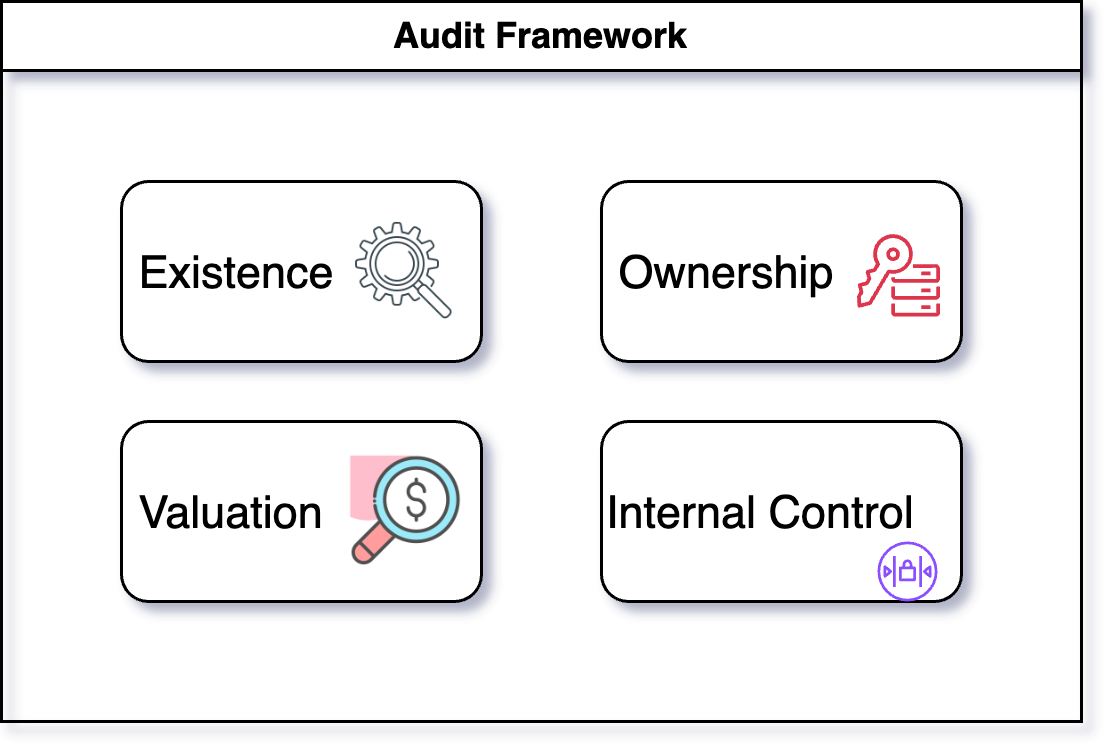
\includegraphics[width=0.9\textwidth]{figures/audit_framework.png}
    \caption[Audit Framework for Cryptoassets]{Audit Framework for Cryptoassets. Simply put, a cryptoasset \textit{exists} when it has a material \textit{value} and is \textit{owned} by an entity. Ownership requires \textit{internal control} to keep the asset accessible and safe.}
\end{figure}	
% https://app.diagrams.net/#G1y7zKo_RABPdLiRYjitMpIwxWSk-9ey47	

We first set out to organize auditing issues into themes and establish a framework for analyzing them. In our paper~\cite{pimentel2021systemizing}, we report on an extensive set of interviews we conducted with auditors at large and medium sized firms. Applying thematic analysis to the interviews, we developed the framework in Figure~\ref{fig:audit_framework}. The framework breaks auditing issue into four themes: existence, ownership, valuation, and internal control. This can generally be applied to any asset, however we consider how it applies to crytoassets specifically below.


\subsection{Existence} \label{sec:auditing:framework:existence}
Auditors need to establish that financial statements, as reported, are free of material misstatements. One area that was repeatedly cited as a challenging area for our respondents was the existence of cryptocurrencies. The main question to answer is whether the reported cryptoassets actually exist. Not all blockchains are created equally, and the reliability of the blockchain is a key consideration. For instance, if all nodes stop operating a blockchain protocol or there are only a few validators, the blockchain could effectively cease to exist. Another challenge is how to verify the existence of a token, where a company is reporting balances of a token that might not exist on any blockchain. 


\subsubsection{Reliability of a Blockchain}

One challenge of auditing the existence of cryptoassets is simply due to their non-physical nature~\cite{pimentel2021systemizing}. Unlike inventory or land that auditors can observe, auditors are required to find alternative evidence for these intangible assets. Evaluating the existence of a cryptoasset necessarily requires relying on a blockchain upon which a cryptoasset resides. Further, determining whether a given blockchain is reliable or not can prove difficult. Although blockchains are touted as immutable, not all blockchains are created equally. Hence, the ability to rely on a blockchain will depend on factors such as the robustness of the consensus mechanism, depth of the community supporting the blockchain, and reliability of the cryptography involved, number of validators, among other things. Consider Bitcoin: there is a large community supporting it, firms are involved, miners devote material hashpower to it, the cryptography and consensus mechanism have been reviewed by experts. The existence of BTC is less questionable than the native currency on an obscure blockchain.

Auditors must be able to evaluate the reliability of the blockchain they are relying on to provide evidence for the existence of cryptoassets. The challenge lies in determining how much work is involved in validating the blockchain itself. Whether a full code review or investigation of the underlying blockchain's cryptography is necessary will be a case-by-case decision. However, this may result in duplicate work if each firm is providing an in-depth review of each blockchain for each mandate. Best practice would involve firms developing a library of blockchains which have been tested (for instance, blockchains for which a code review has been done at a certain date) and which future engagement teams within the firm network can rely on to reduce the duplication of work.

Another challenge remains determining how to rely on transactions that are not on the blockchain. For instance, many exchanges pool or commingle the accounts of several clients. In a secondary ledger (not on the blockchain), they record the positions of each client and then may record offsetting positions of those clients in this secondary ledger and not actually record the exchange on the blockchain.


\subsubsection{Forks and Airdrops} \label{sec:auditing:framework:existence:airdrops}

Existing accounting standards do not contemplate how to account for non-reciprocal transfers of assets like in the case of forks or airdrops. In many cases, the recipient of the tokens often does not have the option to reject the deposits, nor would they get notified of the new tokens received, which could result in issues with completeness. There are practices to address \textit{gifts} in the financial audits, however, it is unclear if Forks and Airdrops are considered gifts, mainly as sometimes there are costs or actions required to claim the tokens. It is worth to mention that also the reliability of the blockchain the new tokens live on is a concern. As an example, in September 2022, with Ethereum switching from Proof of Work to Proof of Stake~\cite{themerge}, the PoW continued to exist as a fork, however, does not have the same level of security and network support as the main chain. Similarly, in August 2017, when a hard fork created Bitcoin Cash from Bitcoin's main ledger, holders of Bitcoin before the fork were assigned Bitcoin Cash in the same amounts. 

% \textblue{Expand a little, focus on existence, forward pointers to other aspects. TODO: add ref to ownership}


\subsection{Ownership}\label{sec:auditing:framework:ownership}

Auditors must be satisfied that the assets reported on the company's balance sheet do in fact belong to the company, or if the client is operating as a custodian for third-parties (for instance, as an exchange who holds cryptocurrencies received from third-parties), that the assets held do in fact belong to the third party who claims to possess them. After establishing existence of the tokens, auditors need to confirm the rightful owner of the assets and verify the company's claims. For traditional assets, firms might overcome the ownership issue in several ways. First, a client can demonstrate ownership of an asset with reference to a generally accepted official document. For instance, a property owner can demonstrate ownership of their building with reference to a deed. However, in a blockchain environment, no central authority exists to produce such official documents. Second, firms may engage a custodian to hold assets on their behalf, like a bank. This does not eliminate the issue of ownership but simply shifts the concern from the firm's audit to the audits of central custodians.

Therefore, addressing whether or not a client maintains ownership over their cryptoassets will depend on whether they hold their cryptoassets themselves (self-custody) or through a custodian. 

\subsubsection{Self-Custody of Assets}
In the absence of legal registers to support ownership or documents bearing the name of the firm, the auditor must rely on the internal controls of the entity to obtain comfort over the ownership assumption~\cite{pimentel2021systemizing}. A question emerges about what ownership means in this context both temporally and in terms of access to a private key. Temporally, auditors must distinguish between whether they are able to provide support for ownership over an asset at the date of conducting the audit procedure or at the end of the fiscal period under audit. For example, if an auditor verifies that a client owns bitcoin one month after year-end through procedures, this proves that the client controlled the asset on that date but says nothing about whether the client owned those assets at year-end. With inventory, in the absence of performing a count at year-end, the auditor may perform roll-back procedures to verify the transactions between the count date and the year-end date to obtain comfort over the year-end balance. To do so, this would require that the auditor ensure that ownership was maintained over the subsequent events period even if this is not what is required by the auditing standards. Here's one of the challenges that was brought up from a financial auditor in our paper~\cite{pimentel2021systemizing}:


\begin{quote}
Do I need to prove that they retained ownership over the subsequent events period? The auditing standard doesn't say that I do. If the client loses ownership during the subsequent events period, do I need to unrecord the whole thing at year-end? Likely, this would be an issue of note disclosure. In the past, this has been used before for some fraud cases, but in those cases, it was because those transactions never really occurred.
\end{quote}

Determining when to test ownership to ensure that evidence is obtained at the correct date becomes a challenge. Best practice would indicate that, like inventory, auditors should test ownership as at the balance sheet date and may wish to provide note disclosure for significant events where ownership is lost. 

A question emerges about what ownership really means in this context. A client may demonstrate that they have access to a private key, but this in and of itself does not demonstrate ownership. ``With ownership, the risk of giving someone else access to the private key is no different from the corporate controller sharing his password to the company bank account with his spouse''. Auditors must determine what types of procedures they can do to validate control and ownership in this context.

If a client uses self-custody, we can do different procedures to be able to approve ownership like small amount transfers or secret messages, depending on the protocol they're using. These practices like small value transfers or the sending of secret messages are part of what are referred to as cryptographic proofs. 

\subsubsection{Cryptographic Keys} 

Although alternative notions of ownership are possible to define, the idea of a signing key is foundational and seen with bitcoin, Ethereum (ETH), and ERC20 tokens. Thus, demonstrating knowledge of this key is necessary, but not sufficient, to demonstrating ownership. The most direct cryptographic technique is to use a so-called zero-knowledge proof of this private key, and to staple in some information identifying the context of the proof. For standard proofs, this is cryptographically equivalent to simply signing a challenge message with the key (See Section~\ref{digital_signature}). Folklore protocols of sending small cash amounts from an allegedly owned account to the auditor to demonstrate control are also commonly noted in the literature. This offers similar security but may add ethical complexities for the auditor in accepting the amount transferred. 

We note that while cryptographic proof is necessary, it is not sufficient. A cryptographic proof simply demonstrates that the purported owner has access to the person holding the signing key. A malicious company might arrange for the owner of cryptoassets to engage in signing statements or moving test amounts fraudulently on their behalf. This issue is not new: an insolvent retail store might borrow inventory from elsewhere to inflate its assets during an inventory count. Auditors mitigate this by arranging a common date for all audits of physical inventory and, similarly, cryptographic audits could be synchronized on a fixed schedule to prevent the same assets from being counted for different companies in different audits~\cite{dagher2015provisions}. 

One type of proof includes sending a small amount (the amount is random challenge) of money to the auditor from the private key, while another proof involves demonstrating that the client can respond to a cryptographically-protected message that only the private keyholder could open. Independently, neither of these procedures demonstrate that the client owns the private key. Effectively, sending a small amount on chain leaves an evidence for the auditor to observe if another entity have access to these keys (or the same company is double counting their assets), however, the digital signature does not leave any on-chain evidence. 

% \textblue{On reflection, I guess there is a difference between off-chain signing, OP\_RETURN or equivalent, and sending small amounts. The second two leave on-chain evidence, while the first does not. So if I am sharing assets with another insolvent entity with different auditors, we are more likely to get caught by the second two methods than the first one.}

It should be noted that due to technical nuances of the cryptographic implementation, this requires tooling to be able to irrefutably verify the validity of the signature by the auditors~\cite{gavinwrightcourt}. However, auditors rely on the sum of several procedures to obtain reasonable assurance over this assertion~\cite{pimentel2021systemizing}: 


\begin{quote}
With ownership, it's not a specific procedure but rather the body of evidence that can be performed by signing messages, by testing internal controls, by understanding how the client protects passwords. The clear expectation of ownership is changing. In a traditional audit, the client represents that they own certain things. We see an invoice and we see that they own it. But did they really pay for it? Was it paid for by another company and consigned to them? We perform several procedures to feel comfortable enough to say that they have ownership at that point in time. Our expectations of what ownership means in this area is evolving.
\end{quote}

Many clients are concerned about self-custody due to security risks over holding their own private keys and are turning to custodians to fulfill this function for them. Auditors must adapt their audit procedures to their clients' unique internal control environments and consider competing sources of evidence before coming to a conclusion about ownership. 

% \textblue{You should also mention TEEs and encumbered keys --- see paper on complete knowledge} TODO: not sure how to fit this in. 

\subsubsection{Third-Party Custodianship}\label{sec:auditing:framework:ownership:custodianship}

In a traditional audit context, the reliance on a third-party custodian is commonplace. Clients might have bank accounts with multiple banks or investment accounts with various brokerage houses. Auditors consider confirmations from these regulated custodians as high-quality evidence. Confirmations in the cryptoasset space are not as straightforward because the entities the auditor would be requesting confirmations from, such as a crypto-exchange, are not always regulated. This raises questions over the reliability of their responses. 

In order to address the reliability of the confirmations from service providers such as cryptocurrency exchanges or other types of custodians, auditors look to the robustness of the internal controls at the service organization. The robustness of these controls is evidenced by the presence of a service organization control (SOC) report. In order to rely on the controls of a service organization such as a payroll provider or investment custodian, auditors often obtain SOC reports, which provide assurance over the processes and data security at the custodian. Two types of reports are available: an SOC 1 report provides assurance over the controls used by a service provider who processes financial data; an SOC 2 report provides assurance on controls over the processing of non-financial data in accordance with Trust Services Criteria~\cite{bdosocreports}. 

While some blockchain firms have been able to obtain SOC reports, the mere fact of having the report is insufficient. Obtaining an SOC report is not a box-checking exercise and that the auditor must review the report carefully to understand which controls it has addressed and can be relied on.


\subsubsection{Forks and Airdrops}\label{sec:auditing:framework:ownership:airdrops}
More commonly for ERC-20 tokens on Ethereum, the recipient of the tokens often does not have the option to reject the deposits, nor would they get notified of the new tokens. As mentioned in section~\ref{sec:auditing:framework:existence:airdrops}, all ETH holders received ETH PoW on the time of the merge~\cite{themerge}, however required new software to access them. However, in some other instances, such as Optimism Airdrop~\cite{allen2023airdrop}, the recipient of the tokens must claim the tokens in order to receive them (See Figure~\ref{fig:opairdrop}). In this case, the auditor must ensure that the client has claimed the tokens, the price of the time of the claim, and the validity of the claim from the client's keys in order to include them in the financial statements.



\subsection{Valuation of Cryptoassets} \label{sec:auditing:framework:valuation}
When values are reported on financial statements, they must be reported in the functional currency of the firm, meaning the primary governmental currency used. A challenge for blockchain entities is to determine the valuation of cryptoassets on the financial statement date or the conversion rate for sales and expenditures made throughout the year. Auditors must be satisfied that the values reported in the financial statements are accurate and represent the underlying economic reality~\cite{eyvaluation}. Following this framework flow, we have verified that the tokens exist, the client has the ownership of the tokens, and now we must determine the value of the tokens are correctly reported by the client. This issue can be considered a subset of the "Oracle Problem" which is discussed further in the context of decentralized applications (DApps) and smart contracts in Chapter~\ref{sec:oracles}, however, the issue discussed here is more related to the valuation of cryptoassets on the financial statements of the company.


\subsubsection{Fair Value of Cryptoassets}
A significant obstacle for obtaining audited financial statements is the determination of a fair value for cryptoassets. Cryptoassets are often difficult to value because it is challenging to determine their underlying value and there may not be a generally accepted, quoted value to use as a reference. As an analogy, firms value foreign currencies at the closing rate on the transaction date, as reported by the central bank servicing the firm's area. No universal central bank offers rates for currency-like cryptoassets. At the time of writing, only a few Fortune 500 financial firms, \eg CME (Chicago Mercantile Exchange), offers a daily reference rate for bitcoin and ether, but not for most cryptocurrencies or cryptoassets.
While bitcoin and ether enjoy around-the-clock trading across many markets, lesser-known coins, tokens, assets, or liabilities may trade slowly, and in low volumes. Generally speaking, low liquidity results in stale last sale prices and large bid-ask spreads. This is challenging but not unprecedented in financial auditing: privately held stocks and over-the-counter financial instruments share a similar profile. Auditors must familiarize themselves with the exchange markets for the cryptocurrencies held by their client to assist in validating their valuation.

\subsubsection{Geographical Variation}
The same cryptoasset might have different market values across different jurisdictions — because of market frictions, arbitrage does not resolve these differences~\cite{kroeger2017law}. If a firm applies International Financial Reporting Standards (IFRS), any financial assets measured at fair value that they hold must be determined with reference to their principal market (if available), which refers to the ``market with the greatest volume and level of activity for the asset''~\cite{ifrs13fairvalue}. Therefore, this standard precludes a firm from using the valuation of a cryptocurrency based on an obscure market price. Auditors will need to look carefully at the record of a client`s trading activity to determine the location of a client`s principal cryptoassets market and ensure that the assets are valued accordingly on the financial statements.


\subsubsection{Fungibility}\label{fungibility}
Fungibility represents a critical yet often overlooked challenge for auditors in the realm of cryptoassets. The concept of fungibility refers to the ability of an asset to be interchangeable with other individual assets of the same type, implying that each unit is indistinguishable from another. In traditional finance, currencies and commodities often embody this principle, where each unit holds the same value and is interchangeable without distinction. However, the digital nature of cryptoassets introduces complexities that can compromise their fungibility, leading to significant implications for valuation and auditing.

A prominent issue in the crypto space is the differentiation between ``dirty'' coins and ``clean'' coins. Dirty coins are those that have been involved in illicit activities or are otherwise tainted by their transaction history, making them potentially less desirable or even subject to seizure and legal action. This contrasts with clean coins, which have no such associations and are freely usable and exchangeable. The case of tainted ETH from now sanctioned Tornado Cash~\cite{ofactornadocash,pertsev2019tornado}, a privacy tool designed to obscure the origins of Ethereum tokens, exemplifies this challenge. Funds with history of being mixed through Tornado Cash are flagged by regulatory bodies and exchanges, affecting their acceptance and fungibility. 

% Moreover, "dusting attacks" further complicate the fungibility of cryptoassets. In such attacks, small amounts of a cryptocurrency, known as dust, are sent to a large number of addresses. This tactic can breach privacy by identifying the owners of those addresses if they move the dust along with other funds, inadvertently linking their wallets. Dusting attacks not only pose privacy concerns but also impact the fungibility of the assets involved, as the dust may be traced back to illegal activities, thereby tainting the recipient's entire wallet.

For auditors, these issues present unique challenges in valuing cryptoassets. The presence of dirty coins, the risk of dusting attacks, and the potential for assets to be tainted by association with privacy tools or illicit activities necessitate careful consideration and due diligence. Auditors must navigate these complexities, employing advanced blockchain analysis tools and staying up to date with regulatory developments to accurately assess the fungibility and, by extension, the valuation of cryptoassets in their audits.



\subsubsection{Forks and Airdrops}
Continuing the airdrop challenges from sections ~\ref{sec:auditing:framework:existence:airdrops} and~\ref{sec:auditing:framework:ownership:airdrops}, if existing accounting standards require the measurement of transactions at historical cost (what was paid for the assets), then recipients of Bitcoin Cash, fork of Bitcoin, would report this new asset on their books at a value of \$0. Certainly, this does not represent the true value acquired through the fork~\cite{webb2018fork}. Commonly, the newly created tokens do not have mature markets, which present another challenge for valuation of these cryptoassets. Therefore, auditors must address the issue of an accounting standard that does not contemplate how to measure the value of cryptoassets when considering whether the financial statements they are reporting on are accurate in all substantial respects.


\subsection{Internal Controls} \label{sec:auditing:framework:internalcontrol}

Following our audit framework, once the existence and ownership of cryptoassets are verified at an established valuation, auditors must shift their focus towards evaluating the effectiveness of the client's internal controls. The nature of internal controls related to cryptoassets is often novel for auditors, characterized by a lack of comprehensive documentation and a tendency towards less secure automation practices. Effective internal controls in the realm of cryptoassets are multifaceted, encompassing operational processes, policies, access controls, continuous monitoring, key management practices, and the underlying IT infrastructure.

A critical aspect of internal controls in the context of cryptoassets involves navigating the trade-off between ownership verification and the robustness of these controls. For instance, more secure internal controls, such as the use of multisig wallets, can complicate the process of proving ownership. While multisig wallets enhance security by requiring multiple parties to sign off on transactions, thus distributing control and reducing the risk of unauthorized access, they also introduce complexity in demonstrating clear asset ownership. Furthermore, using an Externally Owned Account (EOA) simplifies ownership verification but may compromise the effectiveness of internal controls due to the centralized nature of control it entails.

Key management is an essential aspect of internal controls for cryptoassets, necessitating a comprehensive system to safeguard private keys. This system must encompass detailed policies regarding the creation, storage, usage, and recovery of keys. The distinction between cold wallets (offline storage) and hot wallets (online storage) is paramount in this context, with cold wallets offering greater security against hacks at the expense of accessibility. Auditors must evaluate these practices, including who is authorized to execute transactions, how such activities are logged and monitored, and the policies in place to prevent unauthorized access.

Furthermore, the auditor's role extends to assessing the diversity and redundancy of the software and hardware employed to manage and protect these keys. A robust internal control environment for cryptoassets should not only focus on preventing unauthorized transactions but also on ensuring the continuity and recovery of operations in adverse scenarios --Incident Response Plan--. This comprehensive approach to internal controls, from operational policies to technical safeguards, is crucial in mitigating the inherent risks associated with the management and safeguarding of cryptoassets.


\subsubsection{Segregation}

A related issue to the robustness of the internal controls relates to how the custodian segregates the assets in their possession: 

\begin{quote}
We also have heard that many of these custodians are co-mingling or combining assets into a single account or wallet. That muddies the water a bit and it's difficult in some type of SOC reports to understand what they are really doing to maintain a client's assets. There's a chance that there actually are no assets. If you've given your assets to someone else to hold for you, you may think that they still are yours and that they still exist, but that can be difficult to ascertain.
\end{quote}

When evaluating whether they can rely on the representations from a custodian, the auditor should evaluate how the custodian segregates the assets in their possession. 

In short, in order for auditors to validate ownership, their procedures will depend on whether the client has custody of their keys or uses a third-party. Self-custody will depend on the client's internal controls, while reliance on a custodian will depend on the ability to obtain comfort over the reliability of the custodian. Additionally, cryptographic proofs play an important role in the ability to rely on either party. In order to avoid double-counting of keys, an industry standard common date should be arranged to provide a generally agreed upon ``state of the world'' where keyholders can demonstrate ownership. 

One common method is to rely on confirmations from exchanges as a way to corroborate the existence and ownership of the client's assets, since third-party audit evidence is traditionally viewed as the highest quality of audit evidence for addressing these assertions. 

This finding raises two issues. First, auditors believing they could rely on technologists at their firm to compensate for their lack of knowledge. However, having access to expert knowledge is not the same as deploying it. As we have cautioned throughout the paper, it is incumbent on auditors to develop a fundamental knowledge of blockchain technology to be able to leverage the skills of specialized professionals. And this synergy is only possible when auditors and technologists collaborate~\cite{bauer2019one}. Second is the lack of guidance on how to audit cryptoassets. We believe that by providing rigorous sets of standards and through ongoing inspections by audit oversight bodies, a corpus of generally accepted auditing standards for this sector will develop. These standards will provide guidelines that auditors who are not blockchain experts can use when attempting to make inroads into this sector. 




% As discussed in Section~\ref{sec:auditing:framework:ownership:custodianship}, auditors rely heavily on SOC reports to obtain comfort over the internal controls of a custodian. However, SOC reports are not always available, and even when they are, they do not always cover the relevant controls for custody of cryptocurrencies. SOC reports require the company to provide a description of the system, including the controls in place, and the auditor to provide an opinion on the design and operating effectiveness of the controls. However, the SOC report is not a panacea. The auditor must still evaluate the report to determine whether the controls are adequate for the purposes of the audit. Additionally, the SOC report is only as good as the date it was issued. If the SOC report is dated after the balance sheet date, the auditor must obtain additional evidence to ensure that the controls were in place at the balance sheet date.

%TODO: dig deeper here that what the SOC report requires and what it doesn't

\subsubsection{Forks and Airdrops} 

Assuming the auditors previously have verified that the new token exists, it is owned by the client, and it is valued at an established price, furthermore, they need to assess the processes for claiming the airdrop or forked token. This process commonly involved creating a transaction (or signing a message) on a newly created blockchain (smartcontract) and interact with external code. The complexity of this process depends on the technical nuances of the airdrop or fork; however, the risk of losing the main coins is imminent. As an example, in 2016, after the DAO hack~\cite{siegel2016daohack} emergency network upgrade, Ethereum was forked into the ETC (Ethereum Classic), and ETH (Ethereum). Many users lost their ETH after transferring their ETC to another account~\cite{ethereumClassic}, as the blockchains were so similar that transactions could be replayed on the other chain --``replay attack''--. To mitigate this issue some toolings were developed to add \textit{relay protection} to the transactions and the blockchain. 



%++++++++++++++++++++++=======================================+++++++++++++++++++++


\section{Case Studies} \label{sec:auditing:case-studies}

As is quite common in the business academic literature (compared to the computer science literature), we will illustrate a set of auditing issues through a set of case studies.  For each case study, we present a realistic scenario. We then classify the auditing issues based on our framework. Finally, we analyze the case for relevant examples where subtle technical nuances blockchain technology need to be understood, fitting with the theme of the dissertation.

While the case studies are fictitious (unless otherwise noted), they are rooted in real experiences in industry. My personal experiences include, but are not limited to, my role as: a blockchain engineer at the Bitcoin ATM company \textit{Bitaccess}, a senior security auditor at \textit{ConsenSys Diligence}, a chief technology officer (CTO) at the publicly traded company \textit{Ether Capital} which established Canada's first Ethereum ETF. Additional input came from my advisor Jeremy Clark, a research chair sponsored by \textit{Raymond Chabot Grant Thornton}, and from my co-author Erica Pimentel who conducted interviews of auditors for our paper~\cite{pimentel2021systemizing} (see the paper for the description of each interviewee). The case studies do not directly represent any of the companies mentioned above.


\subsection{Case Study 1} \label{sec:auditing:case-studies:existence} % Existence

Optimism is a software project for building a scalable `layer 2' on top of Ethereum. At the time of writing, it represents the second largest layer 2 (next to Arbitrum).\footnote{\url{https://l2beat.com/scaling/summary}, accessed March 2024.} The Optimism~\cite{optimismgithub} team decided to airdrop \texttt{OP} tokens to the Ethereum addresses that met a criterion of activity on the Ethereum mainnet. In this section, we do not discuss what Optimism is, and how it works, and we only focus on the auditing challenges of the airdrop for the auditors and the cryptoasset holders (See Section~\ref{sec:auditing:framework:existence:airdrops}). 

The airdrop was done in two phases. The first phase was done in May 2022, and the second phase was done in February 2023. The first airdrop was done in a way that the recipient of the tokens must claim the tokens, by sending a transaction, in order to receive them. This is different that many previous \textit{push} airdrops, where the recipient of the tokens did not have the option to reject the deposits, nor would they necessarily get notified of the new tokens received (depending on whether their software client was active and configured to report new transactions). 


\begin{figure}[t]
    \centering
% \floatbox[{\capbeside\thisfloatsetup{capbesideposition={left,bottom},capbesidewidth=0.5\linewidth}}]{figure}[\FBwidth]
{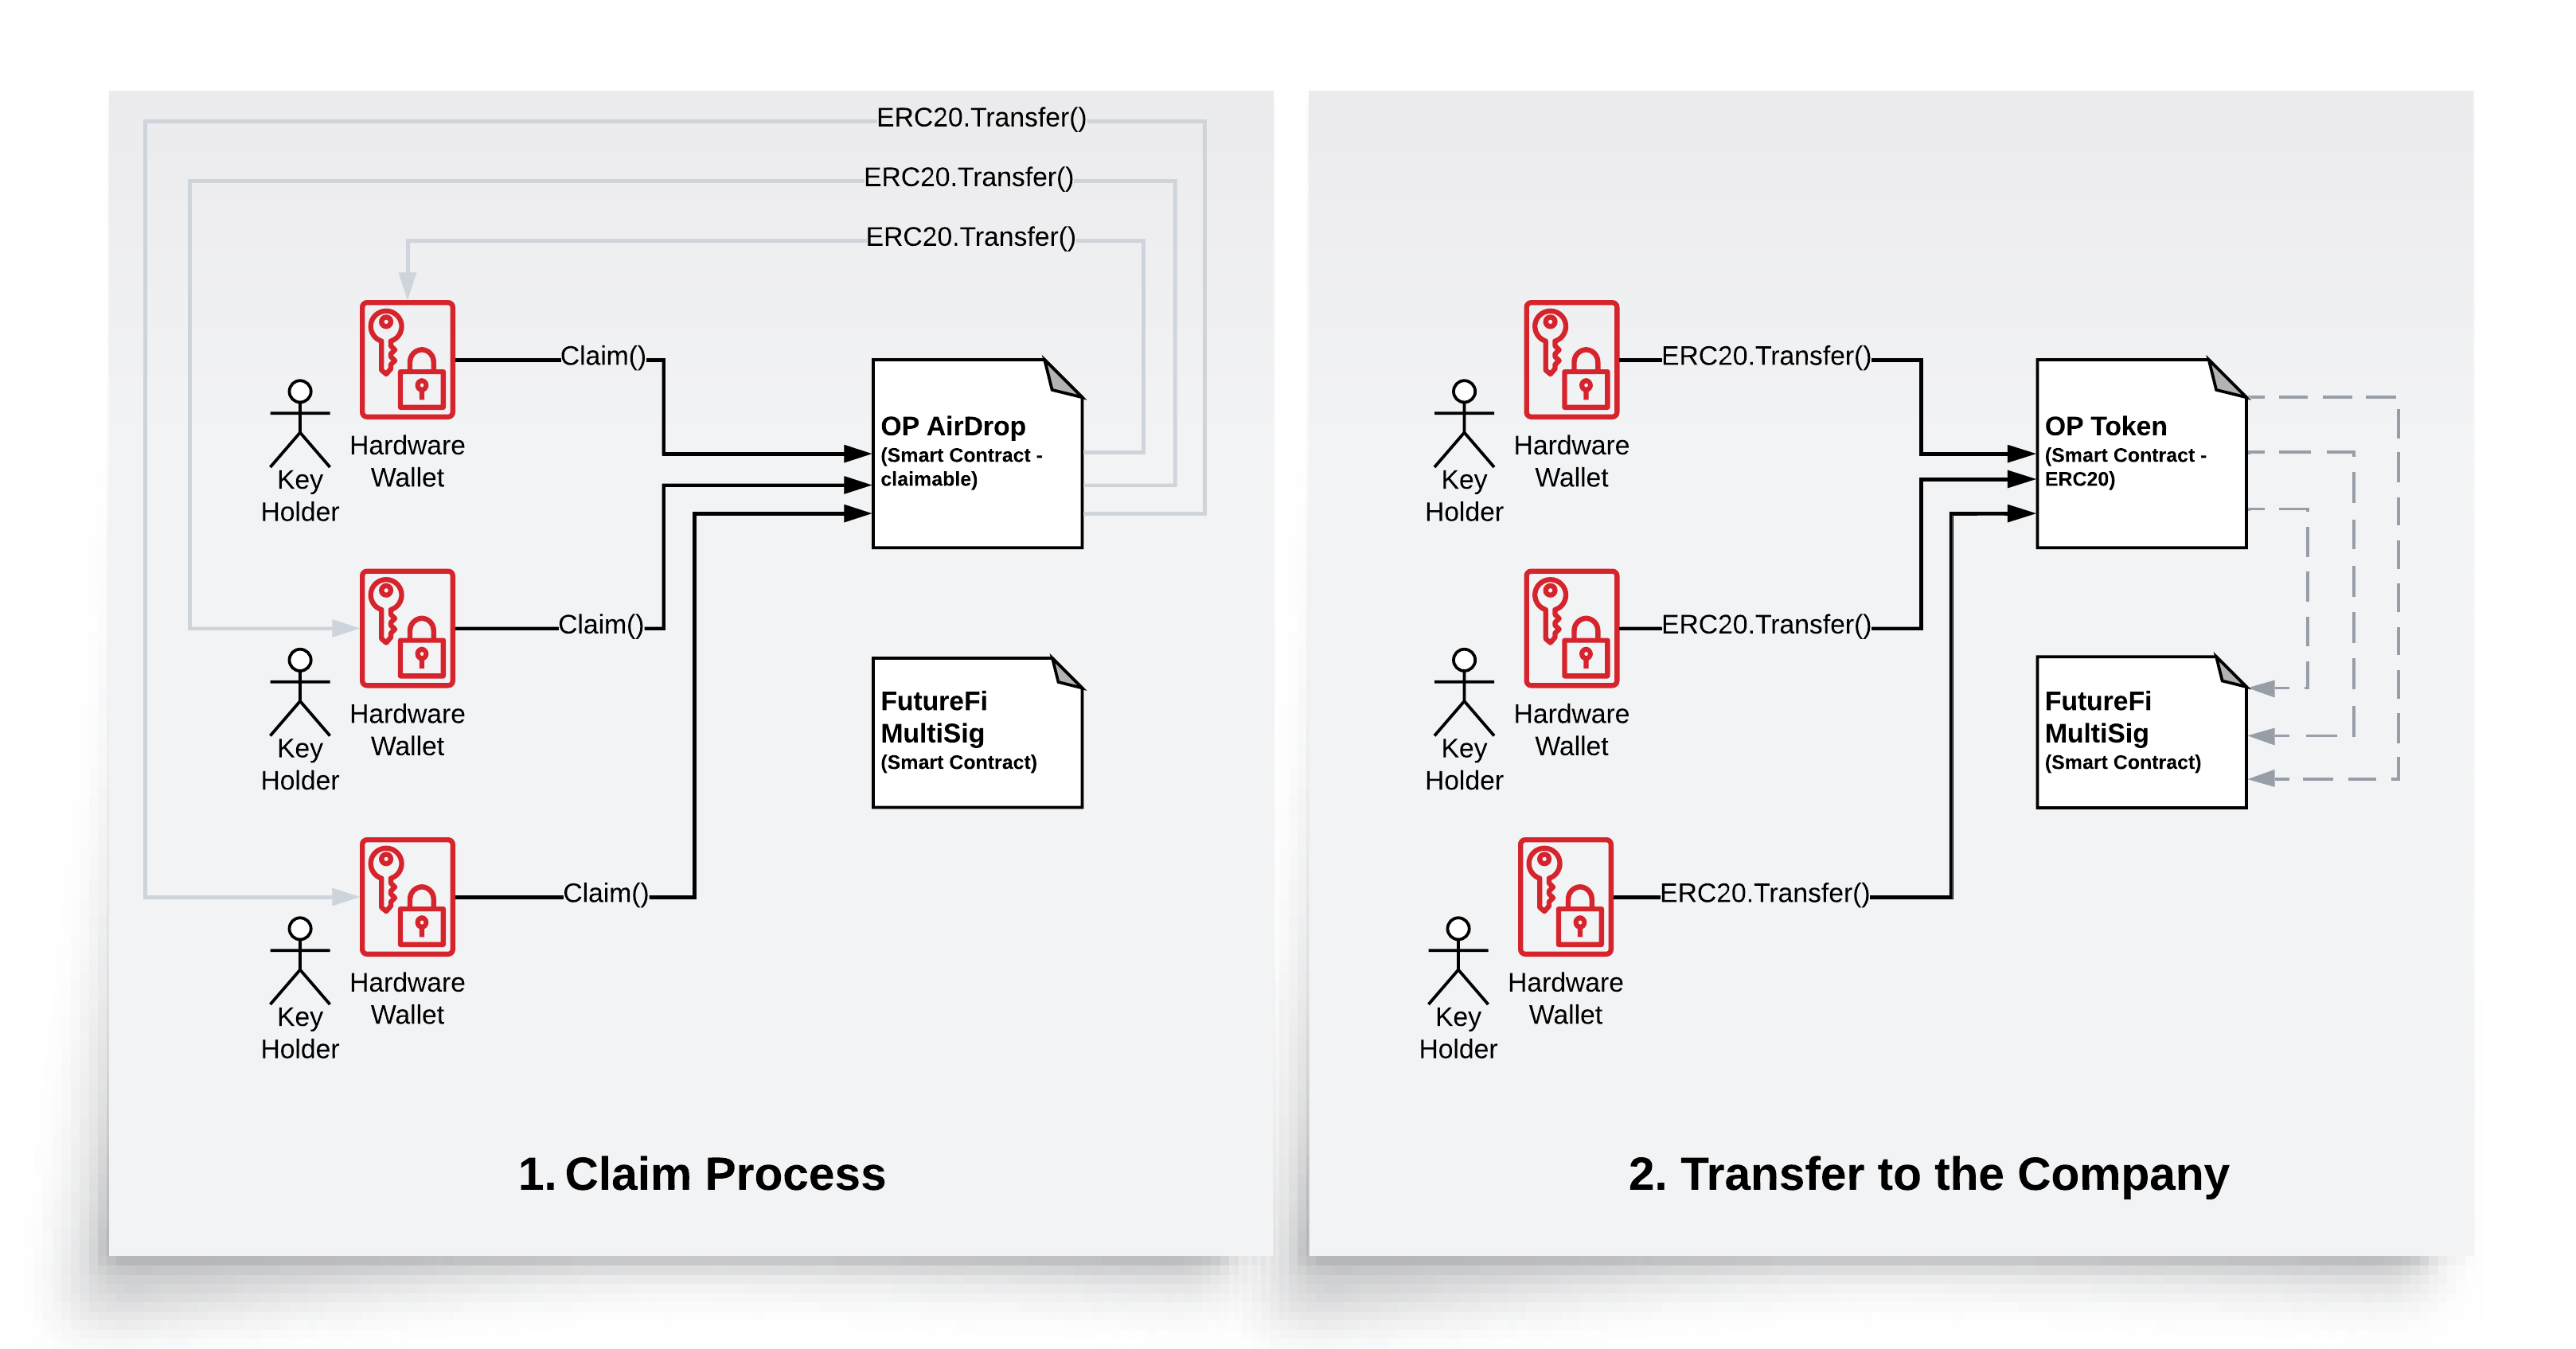
\includegraphics[width=1\textwidth]{figures/BlockchainAudit-OPAirdrop.png}}
{\caption[Case Study 1 - Optimism Airdrop First Claim Workflow]{Case Study 1 - Optimism Airdrop First Claim Workflow for Multisig Custody}\label{fig:opairdrop}}
\end{figure}
%https://lucid.app/lucidchart/b8451756-8053-44ed-8ee2-309b7e51e2e7/edit?view_items=N._4KqjqwzbO%2C9o_4DOb.NPth%2CJ._4oQuPEYwQ%2C3y_4TU90WCu2%2Cdc.4QL7K-l~o%2Ci~_4v5aBkjN1%2Cs~_4BWduTZcZ%2Co~_4Rnr3RJ40%2CTa.4miSeusA~%2Cea.4uKkej.BX%2C2~_4Ry82OCpe&invitationId=inv_5d90099c-1dd3-4f9d-825a-b3fe6c85c14d
%

\paragraph{Classification.} This case study mainly is focused on the ~\textit{existence} (See Section~\ref{sec:auditing:framework:existence}) of the tokens and how the auditor must develop a procedure to ensure that the tokens have been claimed, transferred, and accounted for in the financial statements. However, such as the valuation of the tokens, and the internal controls of the client (in the claim process) are also important factors that must be considered by the auditor.

\paragraph{Analysis.} 

There are some technical nuances that are worthy of mentioning. Assume a company has a multisig smart contract account as their main address, and 10 keyholders for the multisig smart contract (the threshold here does not matter). Each of the keyholders were included in the recipients list of the airdrop. In order for the company to receive the airdropped tokens, each of the keyholders must claim the tokens by sending a transaction (See Figure~\ref{fig:opairdrop} for more details). For normal use of the multisig smart contract (\eg Gnosis Safe), the keyholders do not require any Ether balance to pay for gas, however this transaction requires an onchain transaction and gas. After the claim process is done, the tokens required to be transferred to the main address of the company, which required more gas to be paid. This process is cumbersome and requires manual review of the transactions to ensure the correctness of the process. To make the matter more complicated, the airdrop was done in two phases\footnote{There were three consecutive airdrops, however, for the sake of simplicity in this case study, we will focus only on the first two, as the second and third airdrops were technically identical, rendering the examination of the third phase redundant.}, and the second phase was done after the first phase was completed and only airdropped to addresses that have claimed and participated with the governance of the Optimism protocol~\cite{allen2023airdrop}. The second phase of the airdrop did not need to be claimed and was sent to the eligible addresses, which made the auditing process more complicated and different from the first phase. 

In here we assume all the technical details of the claim process has been handled by the technical team of the company, and the auditor only needs to ensure that the tokens have been claimed. It should be noted that this process by itself is not defined in the auditing standards or procedure and is a novel process that the auditor must develop a procedure for. In order to audit the existence of the airdropped tokens, the auditor must ensure that the client has claimed the tokens, the cost of the claim (gas), and the price of the time of the claim, in order to include them in the financial statements.  This process is not straightforward and requires manual auditing of the client's Ethereum addresses. Additionally, the auditor must ensure that the client has claimed the tokens before the end of the fiscal year, otherwise the tokens must be excluded from the financial statements. There are many open challenges in this process, as each transfer of tokens requires to be recorded and explained in the audit report. Additionally, many of these airdropped tokens, are not listed on any exchanges or have really low valuation to be considered material, hence the auditor must rely on the client's internal valuation of the tokens. 

% TODO: (ask jeremy) Another unknown factor here, is the ``participation in the governance'' of Optimism, which is by itself not defined, as it requires more transactions to cast the vote or select a governance delegate in order to be eligible for the second airdrop. This process requires more gas (has costs), and can impact the result of a governance vote. The latter, falls outside the normal audit procedure and requires more technical expertise to be able to audit. 






\subsection{Case Study 2} \label{sec:auditing:case-studies:ownership} % Proof of Ownership
Sean, the CTO of a publicly traded company, is preparing for the year-end audit of the company's financial statements. The company holds a significant amount of cryptoassets, and the auditor has requested proof of ownership of the cryptoassets. The company holds all the cryptoassets in a hardware wallet~\cite{EBSC15} stored in a safe deposit box at a bank. Sean, using the hardware wallet, with auditors as observers, creates a message based on the day's newspaper headline, and signs the message using the hardware wallet. The auditor, using the public key of the hardware wallet, verifies the signature and confirms the ownership of the cryptoassets.

In the following year, Sean upgrades the security of the company infrastructure by moving the cryptoassets to a multisignature smart contract. The keyholders are part of the management and another part board members, separated by responsibility and geographical locations for added security~\cite{c4ccssa}. 

The following quarter, the auditors ask for proof of ownership of the cryptoassets and expect the similar procedure as the last year. However, the company has moved the cryptoassets to a multisignature smart contract, and the auditors must develop a new procedure to be able to verify the ownership of the cryptoassets, as the technical details of the custody has significantly changed. 

\begin{quote}
	\textit{One of our first considerations as it relates both existence and ownership is just to think through how the entity is maintaining custody of their assets. And in particular, what's the security mechanism around access to the private key? Which can vary from being held [in many ways] from online to some type of hot storage to on a piece of paper somewhere, to in a software tool that is not connected to the internet and kind of offline. Which of course, brings down the risk of it being hacked but then increases the risk of physical loss of the private key. We want to understand what our potential clients are doing related to that. Then, as many of them seem to do, we start to gather that they're using a third party around custody.}~\cite{pimentel2021systemizing}
\end{quote}

For the new year audit, almost none of the previous procedures can be reused, mainly due to the fact that previous year's audit, the premise of the ownership of the assets, where based on proof of the access to the private key (\eg signing a message, See Section~\ref{sec:auditing:framework:ownership}). Nonetheless, the new year's audit, includes similar procedure for each keyholder, and a separate procedure for the multisig smart contract which includes many technical nuances.

\paragraph{Classification.} This case study mainly is focused on the ~\textit{proof of ownership} (See Section~\ref{sec:auditing:framework:ownership}) of the cryptoassets and how the auditor must develop a unique procedure based on the technical details of how the company custody their cryptoassets. Also this process is fairly technical and requires in depth knowledge of the cryptographic and blockchain tooling, and the smart contract implementations. There are also many factors regarding the internal controls of the client that must be considered by the auditor, such as how the keys (for each keyholder) are generated, how they are backed up and stored, and the multisig deployment.


\paragraph{Analysis.} As described in Section~\ref{sec:auditing:background}, multisig smart contracts are commonly used by companies to securely store their cryptoassets. Unlike EOA addresses, smart contracts do not have a private key associated with them, hence the proof of ownership cannot be done using the digital signature verification. One approach is to fall back on the older method of transferring a small amount of the asset from and back to the smart contract address. Another is to prove the ownership by verifying the code of the smart contract and then only verify the signatories of the multisig smart contract. This process is more complicated and requires manual auditing of the smart contract code and variables. Additionally, the smart contract can be upgraded or the signatories of the multisig smart contract can be changed at any time, hence the proof of ownership must be done at the time of every audit, and manually verified by technical experts. 



\subsection{Case Study 3} \label{sec:auditing:case-studies:valuation} %  3: Valuation
Bob is the CTO of a company holding cryptoassets named \textit{FutureFi}. He believes the future of auditing is access to \textit{Real-time Financial Reporting (RFR)}, and he wants to be one of the first companies to implement real-time financial reporting and auditing (See Figure~\ref{fig:RFR}). Bob has developed a system that allows the auditors (or any other entity) to fetch the quantity of the cryptoassets held by the company from a blockchain full node and the valuation of the cryptoassets is done using a decentralized price feed as the oracle (See Chapter~\ref{sec:oracles}). This new system replaces the previous procedure of relying on the internal records of the company or use of third party block explorers. The previous methods of obtaining the quantity of the cryptoassets held by the company were prone to errors and software bugs that might have been challenging to identify without rigorous manual review of the code. 


\begin{figure}[t]
    \centering
% \floatbox[{\capbeside\thisfloatsetup{capbesideposition={left,bottom},capbesidewidth=0.5\linewidth}}]{figure}[\FBwidth]
{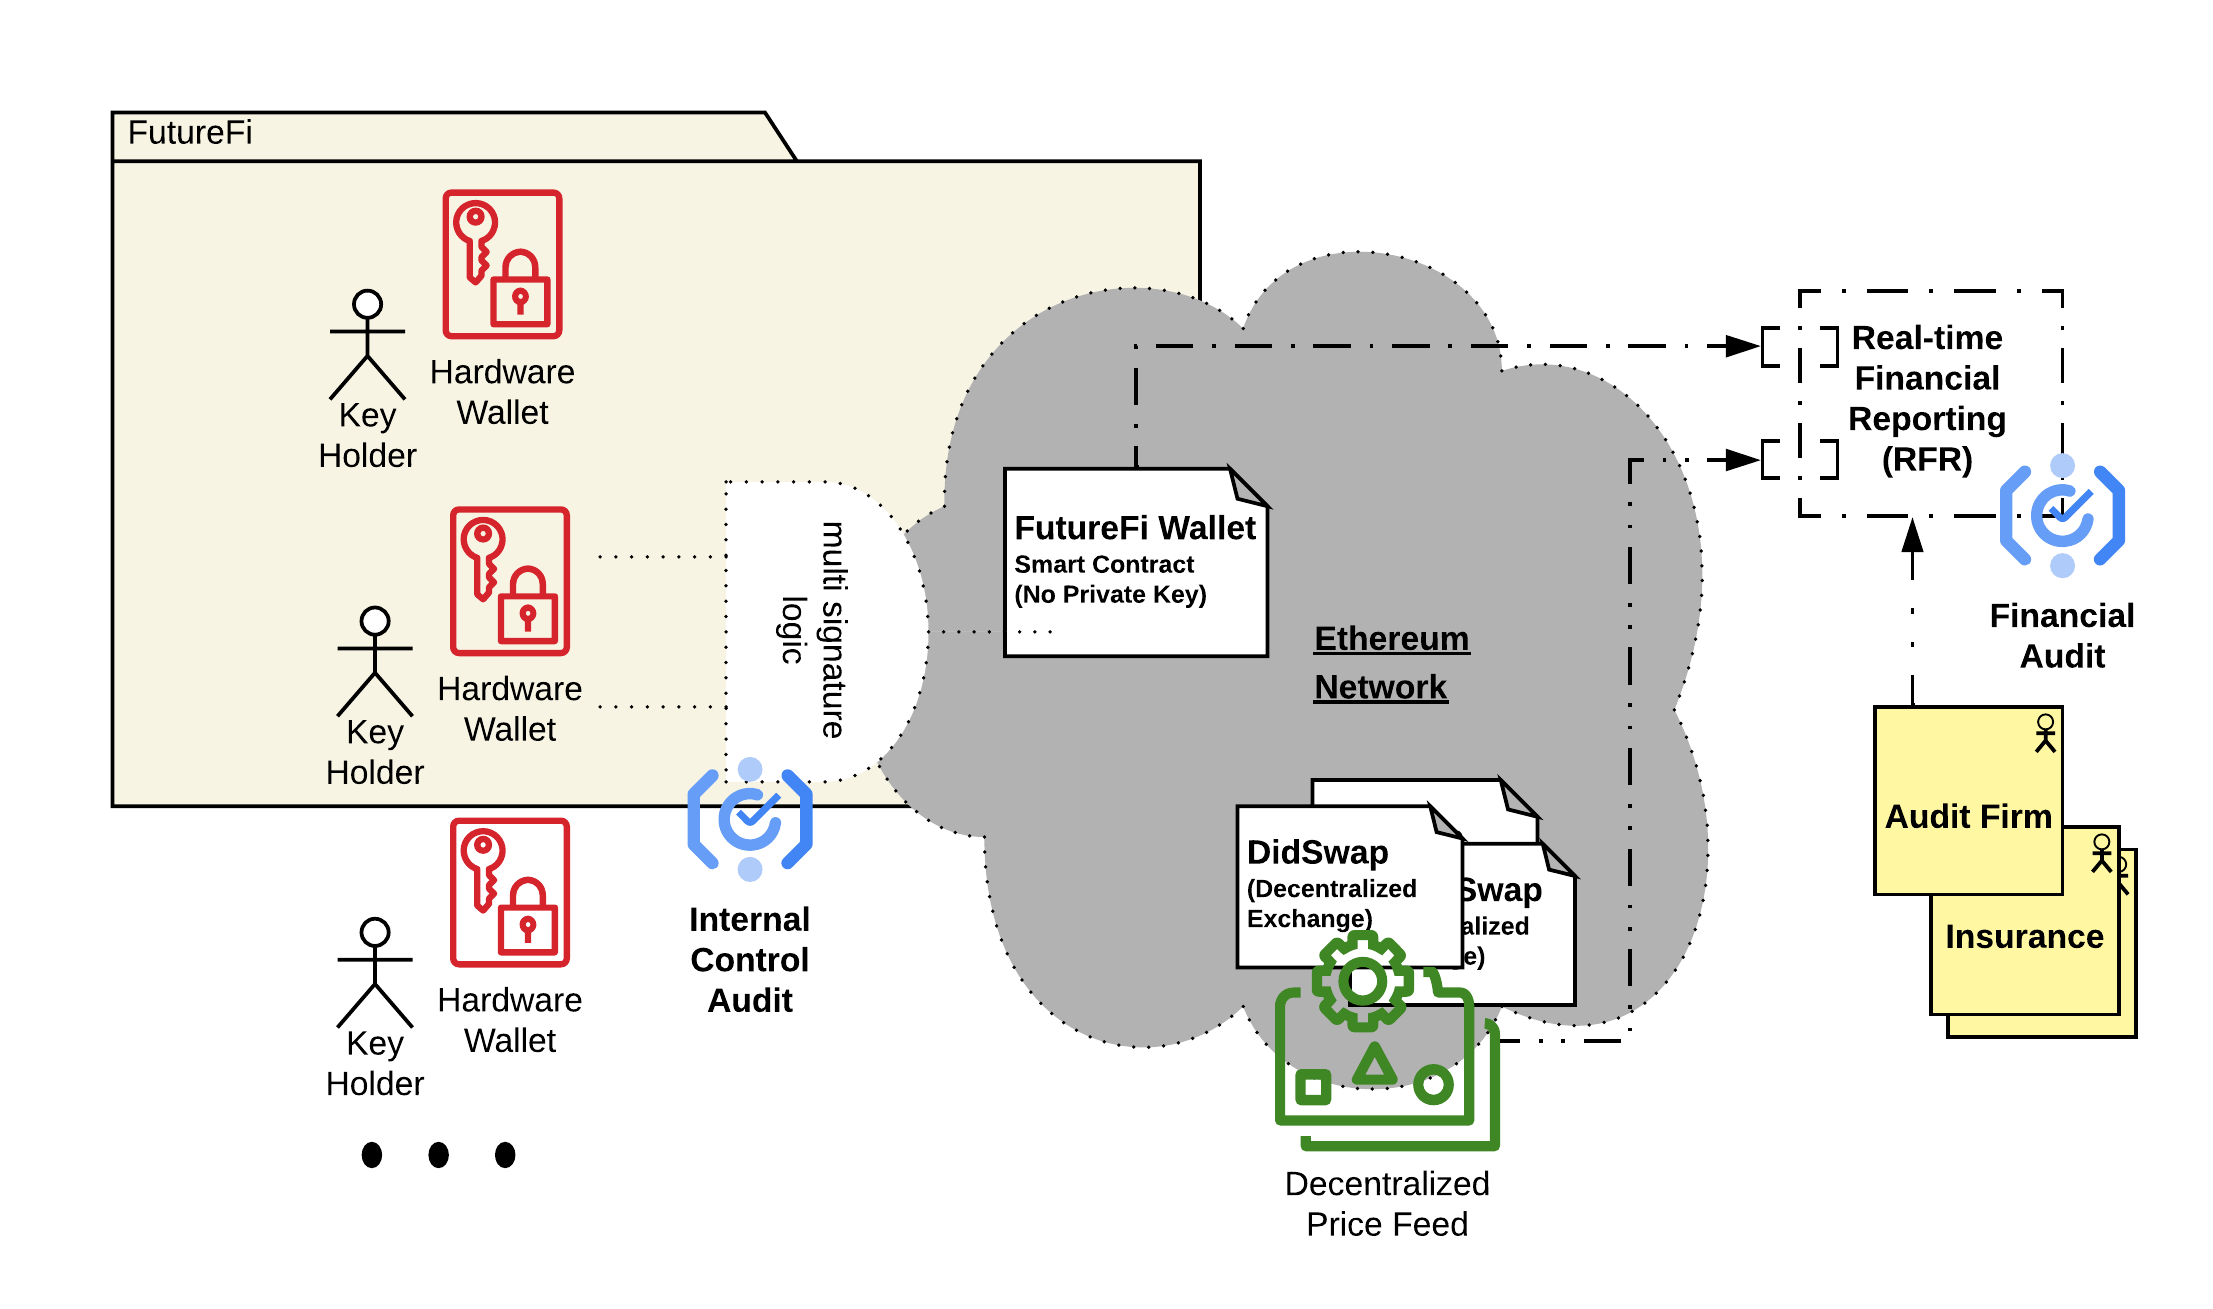
\includegraphics[width=1\textwidth]{figures/BlockchainAudit-FutureFi.png}}
{\caption[Case Study 3 - FutureFi Real-time Financial Reporting (RFR)]{Case Study 3 - FutureFi Real-time Financial Reporting (RFR)}\label{fig:RFR}}
\end{figure}
% https://lucid.app/lucidchart/7ec50abb-44fe-4943-8693-4f89b61df5f9/edit?invitationId=inv_e27c36d0-4434-4b0f-89ae-969703162d5d


Bob's new system allows the auditors to fetch the quantity of the cryptoassets held by the company directly from the blockchain using their own (or trusted) node infrastructure with high degree of confidence. Additionally, the system allows the auditors to fetch the price of the cryptoassets from a decentralized price feed (Such as a Decentralized Exchange), which is mainly more transparent and in some extent more reliable than the centralized price feeds. Centralized price feeds are prone to manipulation and errors with no audit trail, possibly have downtime or delays, and are not transparent. The auditors are satisfied with the new system and the company is one of the first companies to implement real-time accounting and auditing. 

\paragraph{Classification.} This case study mainly is focused on the ~\textit{valuation} (See Section~\ref{sec:auditing:framework:valuation}) of the cryptoassets and how the auditor must develop a procedure to ensure that the price feed is reliable and not manipulated. Additionally, the auditor must validate the real-time financial reporting implementation for any accounting errors and review the internal control of how the quantity of cryptoassets and the price is fetched and included in the financial statements. We believe there are merits in real-time financial reporting standardization~\cite{bakarich2020use,yu2018blockchain} that can benefit both the auditors and the clients, however, the technical nuances of the implementation could result in unforeseen challenges for the accurate reporting of the financial statements. Dai~\etal~\cite{dai2017toward} raise the potential for the blockchain to support the audit function by enabling continuous assurance. 


\paragraph{Analysis.} In such scenario, the auditing process is more efficient and less prone to errors, as the auditors do not need to rely on the client's internal records for the quantity of the cryptoassets held by the company. However, this scenario is not without its own challenges. For example, the auditors must ensure that the price feed is reliable and not manipulated. Additionally, the auditors must ensure that the price feed is not delayed, as the price of the cryptoassets can fluctuate significantly in a short period of time. Any mistake in the price feed can result in significant changes in the audit snapshots, which can make the company insolvent for a short period of time. Any oracle manipulation attack, explained further in Chapter~\ref{sec:oracles}, can result in either over or under valuation of the cryptoassets, resulting in an inaccurate financial statement.




\subsection{Case Study 4} \label{sec:auditing:case-studies:internalcontrol} %: Internal Controls
Ian is an auditor working in one of the big 4 auditing firms. He is assigned to audit a company holding cryptoassets. This company uses a multisig smart contract to custody their cryptoassets. The multisig smart contract is a 2 of 3 multisig smart contract, and the signatories are the CEO, the CFO, and the CTO of the company. The company has acquired a SOC1 report from their custodian, and Ian is satisfied with the internal controls of the custodian. However, the company has a multisig smart contract, and Ian must ensure that the internal controls of the multisig smart contract are adequate. Ian is not familiar with the technical details of the multisig smart contract, and he must rely on the expertise of the company's technical team to ensure that the internal controls of the multisig smart contract are adequate.

To expand on the example, SOC1 report consist of two parts~\cite{RCGTsocreport}, the description of the system, and the auditor's opinion on the design and operating effectiveness of the controls. The description of the system includes the controls in place, and the auditor's opinion is based on the description of the system. However, the SOC1 report is not a panacea. The auditor must still evaluate the report to determine whether the controls are adequate for the purposes of the audit. In this scenario, Ian might consider asking for SOC2 report, as it might be more appropriate. SOC2 provides assurance over controls of the processing of non-financial data in accordance with Trust Services Criteria~\cite{bdosocreports}, which might be more relevant to the internal controls of the multisig smart contract, and mainly the procedure of how each new transaction is signed by the keyholders (\eg outgoing transaction authorization). 

\paragraph{Classification.} This case study mainly is focused on the ~\textit{internal controls} (See Section~\ref{sec:auditing:framework:internalcontrol}) of the cryptoassets custody and key management. SOC reports that are commonly use can ensure the basics of the internal controls and security, however, technical nuances around key management and smart contract security are not covered by such reports. We believe there are merits in adopting standards, such as the C4 Cryptoasset Security Standard Audit~\cite{c4ccssa}, by the big 4 auditing firms, as it is a more appropriate standard for the internal controls of the cryptoassets. CCSS standard includes review of the private key generation process, secure backups, the multisig setup, and manual audit of the multisig implementation and source code. 

\paragraph{Analysis.} As described in Section~\ref{sec:auditing:framework:internalcontrol}, auditors must be satisfied that the internal controls of the client are effective. This is done by testing the design and operating effectiveness of the internal controls. In the context of cryptoassets, this is challenging because the adequate internal controls are novel to the auditors, and the expertise to evaluate and test these controls are not always available. Even if the company has acquired their SOC reports, it is still not sufficient to assume the adequacy of the internal controls. There are better suited standards that test the appropriate checks and balances for the internal controls of the cryptoassets, such as the C4 Cryptoasset Security Standard Audit~\cite{c4ccssa}. However, these standards are not adopted by any of the big 4 auditing firms at the time of the writing. 


%++++++++++++++++++++++=======================================+++++++++++++++++++++
\section{Discussion} \label{sec:auditing:discussion}
% what is the connection between them
To enumerate the points discussed in section~\ref{sec:auditing:case-studies}, we can see that the auditing process of the cryptoassets is not straightforward and requires technical expertise with a deep understanding of the auditing standards and procedures. This is a rare combination of skillets that is not common in the auditing industry. This is a challenge for the auditors, as they must develop a unique procedure for each client, and the lack of standardization can result in errors and mistakes in the auditing process.

Blockchain and smart contracts are labeled as \textit{trustless}, however, the trust is in the code and the protocol to be implemented and executed according to the specification~\cite{gaggioli2019middleman}. The technical nuances that can be introduced by different implementation of the same concept, makes the auditing process more complicated and requires more technical expertise on the specific cryptoasset, smart contract, and the blockchain under audit.

As we pointed out in the previous section, there are standards, such as the C4 Cryptoasset Security Standard Audit~\cite{c4ccssa}, that can be used by the auditors to ensure the adequacy of the internal controls of the cryptoassets. However, as noted, the audit of the cryptoassets require more technical knowledge of the field than previously required on traditional audits, where relying on third party statements were sufficient. This is as if every auditor requires to become a blockchain (smart contract) security auditor as the task of auditing the cryptoassets requires verifying the technical details of the implementation and the code.

\subsection{Paths Forward} 

We will now look at the different paths forward that auditing firms have taken in the past~\cite{pimentel2020blockchain,garanina2022blockchain}, and how it is evolving over time with the maturity of the ecosystem.

\begin{figure}[t]\label{fig:pathsforward}
    \centering
    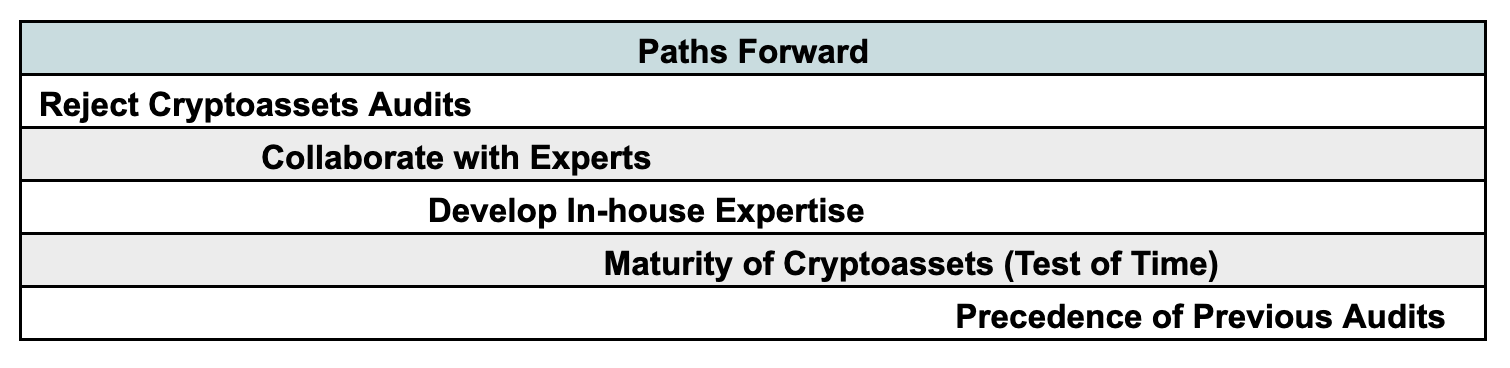
\includegraphics[width=0.9\textwidth]{figures/audit_pathsforward.png}
    \caption[Paths Forward for Auditing Cryptoassets]{Paths Forward for Auditing Cryptoassets}
\end{figure}	
% https://docs.google.com/spreadsheets/d/1fTopz23FVOuOzoLFeYXS3wu6sKbRqPvZiryv0P-T5oo/edit?usp=sharing


\paragraph{Reject cryptoasset audits:} auditing firms can \textit{reject cryptoasset audits} as they have done in early days due to their unknown risk models. This was the case with the early days of the internet, where the auditing firms were not comfortable with the risk models of the internet companies, and rejected the audits. Similarly, many early companies trying to get audited, were rejected by the auditing firms, as they were not comfortable with the risk models of the cryptoassets, and it's been ongoing since. One recent example is Binance, one of the biggest cryptocurrency exchanges, was rejected by the auditing firms in 2022~\cite{binanceauditorrejection}, to conduct a proof-of-reserves audit~\cite{dagher2015provisions}.

\paragraph{Collaborate with experts:} as it has been the case, audit firms can \textit{collaborate with experts} in the field to sign off on the risk assessment of the cryptoassets in question. There is significant research and development in the field of blockchain security and smart contract audits, which can be utilized to ensure the adequacy of the internal controls and work flow of each cryptoasset~\cite{krakenproofofreserve}. Additionally, methods such as formal verification~\cite{clark2018sok8}, can be used to ensure the correctness of the smart contracts and the implementation of the cryptoassets underlying technology. 

\paragraph{Develop their own expertise in-house:} the auditing firms started to \textit{develop their own expertise in-house} and create their own standards, tools, and procedures for auditing the cryptoassets~\cite{eyInternalTools,delloiteinternalauditor}. This is a challenging task, as it requires significant investment in the field (R\&D), and the auditing firms must be able to attract and retain the talent required for such task. Many of the blockchain security firms have hard time finding talent, and the auditing firms are facing the same challenge. 

\paragraph{Test of time:} the \textit{maturity} of the cryptoassets themselves can result in more confidence in the security of the underlying technology (Test of Time), such as the case with Bitcoin and Ethereum. As the cryptoassets mature in the market capitalization, demand, development, and the underlying technology, more banks~\cite{azar2022financial,bankofenglandmaturity}, regulators~\cite{govofcanadamaturity,treasury2023future}, and auditing firms~\cite{kpmgadoption} started to recognize the importance of the cryptoassets and started to research further into the field~\cite{basel2021prudential,drozdz2023mature}. 

\paragraph{Rely of precedence of previous audits:} As more companies are holding cryptoassets, and more audit firms look into these cryptoassets, the auditing process will become more standardized and can be built on top of the previous experiences and reports~\cite{cpabauditingcrypto,han2023accounting}. Integrating standards such as the C4 Cryptoasset Security Standard Audit~\cite{c4ccssa} and security audit procedures, can result in more efficient auditing process for the future audits.




% what do you do about it? 
% - formal analysis, static analysic, manual audits
% - within the manual audit, how to do it?
%     - relavant to rest of the chapter
% - pick up on the technical neuances 
%     - How do you expect furture 500 companies to get the details?


% a bunch of papers on washtrading —> volume issue, not really valuation but you can increase the volume, increase the reputation and hence increase the valuation. not really
% —> assets with no liability


%++++++++++++++++++++++=======================================+++++++++++++++++++++
\section{Conclusion} \label{sec:auditing:conclusion}

This chapter has aimed to demonstrate that, in comparison to traditional audits, audits of clients who hold material amounts of cryptoassets are complex but not impossible. Once a client has been accepted, the three most cited stumbling blocks to providing an audit opinion are the existence, ownership, and valuation of cryptoassets. However, we argue that these issues are not insurmountable if industry guidelines are put into place to allow auditors to verify their client's cryptographic keys against a ``state of the world'' at a generally accepted point in time. Verifying existence and ownership largely hinges on an auditor's ability to verify the possession of cryptographic keys. However, the auditor must be certain that these keys in fact belong to the client and do not simply represent access to an account. Once ownership has been proven, the auditor can rely on the immutable properties of the blockchain to verify existence as the blockchain provides the entire record of transactions since the blockchain's inception. The issue of key sharing is important but is not unlike a situation in the real world where a related party could give the entity under audit a large sum of cash to hold at year-end and report on their financial statement to buoy their financial performance. Volatility complicates the valuation of altcoins and other coins with low trading volumes. However, many other exotic securities exist where accountants rely on complex financial modeling to determine a price.

In sum, this chapter argues that although auditors are rightly cautious when approaching a new sector where clients have not been initiated to the importance of internal controls and where numerous frauds have recently been perpetrated, audits are possible. Additionally, by collaborating closely with blockchain experts and security auditors, auditors who themselves are not experts in blockchain technology can come to a place where they can provide assurance to this sector.




